
\subsection{Modelos utilizados}\label{sec:modelos_utilizados}

Se van a definir las arquitecturas de los modelos usados en el estudio y a justificar su elección.

\subsubsection{DeepConvNet y ShallowConvNet}


Las arquitecturas DeepConvNet y ShallowConvNet, propuestas por Schirrmeister et al. \cite{schirrmeister_DeepLearning2017}, fueron de los primeros modelos convolucionales en lograr un impacto significativo en la clasificación de señales \acrshort{eeg}. Desde entonces, estas arquitecturas han sido ampliamente utilizadas como referencia en numerosos trabajos relacionados con interfaces cerebro-computador y Deep Learning aplicado a EEG \cite{kollod_DeepComparisons2023}.

La arquitectura DeepConvNet está formada por cuatro bloques convolucionales seguidos de operaciones de \textit{max-pooling} y una capa final de clasificación \textit{softmax}. El primer bloque convolucional fue diseñado específicamente para adaptarse a las características de las señales EEG, las cuales presentan un número elevado de canales de entrada correspondientes a los distintos electrodos. Para ello, el bloque es separado en dos capas. La primera realiza un filtrado temporal sobre la señal de cada canal, permitiendo extraer patrones relacionados con las frecuencias presentes en el \acrshort{eeg}. Posteriormente, la segunda convolución aplica un filtrado espacial combinando la información obtenida en la primera capa. Esta separación entre convolución temporal y espacial actúa además como una forma implícita de regularización, forzando a la red a aprender transformaciones más estructuradas \cite{schirrmeister_DeepLearning2017}.


\begin{table}[H]
    \centering
    \footnotesize
    \begin{tabular}{clcccll}
        \toprule
        \textbf{Block} & \textbf{Layer} & \textbf{\# filters} & \textbf{Size} & \textbf{\# params} & \textbf{Output}   \\
        \midrule
        1              & Input          & --                  & --            & 0                  & \((27, 400, 1)\)  \\

                       & Conv2D         & 25                  & \((1,8)\)     & 225                & \((27, 393, 25)\) \\

                       & Conv2D         & 25                  & \((27,1)\)    & 16900              & \((1, 393, 25)\)  \\

                       & BatchNorm      & --                  & --            & 100                & \((1, 393, 25)\)  \\

                       & Activation     & --                  & ELU           & 0                  & \((1, 393, 25)\)  \\

                       & MaxPool2D      & --                  & \((1,2)\)     & 0                  & \((1, 196, 25)\)  \\

                       & Dropout        & --                  & --            & 0                  & \((1, 196, 25)\)  \\
        \midrule

        2              & Conv2D         & 50                  & \((1,8)\)     & 10050              & \((1, 189, 50)\)  \\

                       & BatchNorm      & --                  & --            & 200                & \((1, 189, 50)\)  \\
                       & Activation     & --                  & ELU           & 0                  & \((1, 189, 50)\)  \\

                       & MaxPool2D      & --                  & \((1,2)\)     & 0                  & \((1, 94, 50)\)   \\

                       & Dropout        & --                  & --            & 0                  & \((1, 94, 50)\)   \\
        \midrule

        3              & Conv2D         & 100                 & \((1,8)\)     & 40100              & \((1, 87, 100)\)  \\

                       & BatchNorm      & --                  & --            & 400                & \((1, 87, 100)\)  \\

                       & Activation     & --                  & ELU           & 0                  & \((1, 87, 100)\)  \\

                       & MaxPool2D      & --                  & \((1,2)\)     & 0                  & \((1, 43, 100)\)  \\

                       & Dropout        & --                  & --            & 0                  & \((1, 43, 100)\)  \\
        \midrule

        4              & Conv2D         & 200                 & \((1,8)\)     & 160200             & \((1, 36, 200)\)  \\

                       & BatchNorm      & --                  & --            & 800                & \((1, 36, 200)\)  \\

                       & Activation     & --                  & ELU           & 0                  & \((1, 36, 200)\)  \\

                       & MaxPool2D      & --                  & \((1,2)\)     & 0                  & \((1, 18, 200)\)  \\

                       & Dropout        & --                  & --            & 0                  & \((1, 18, 200)\)  \\

                       & Flatten        & --                  & --            & 0                  & \((3600)\)        \\
        \midrule

        Classifier     & Dense          & --                  & --            & 7202               & \((2)\)           \\

                       & Activation     & --                  & softmax       & 0                  & \((2)\)           \\

        \bottomrule
    \end{tabular}
    \caption{Arquitectura DeepConvNet utilizada.}
    \label{tab:deepconvnet_architecture}
\end{table}

Por otro lado, la arquitectura ShallowConvNet fue diseñada específicamente para la clasificación de características de la potencia de banda. Su estructura busca aproximarse al funcionamiento del método \acrshort{fbcsp} mediante operaciones equivalentes implementadas mediante capas convolucionales. Al igual que DeepConvNet, las primeras capas realizan convoluciones temporales y espaciales. Sin embargo, en este caso la convolución temporal utiliza kernels de mayor tamaño con el objetivo de capturar mejor la información frecuencial de la señal.

Después de estas convoluciones, ShallowConvNet incorpora una secuencia de operaciones compuesta por una \textit{no linealidad cuadrática}, una capa de \textit{mean-pooling} y una activación logarítmica. Este conjunto de transformaciones es análogo al cálculo de la varianza logarítmica utilizado tradicionalmente en \acrshort{fbcsp}. Además, el uso de múltiples regiones de \textit{pooling} dentro de un mismo ensayo permite a la red aprender variaciones temporales de la potencia de banda a lo largo del tiempo \cite{schirrmeister_DeepLearning2017}.


\begin{table}[H]
    \centering
    \footnotesize
    \begin{tabular}{clcccl}
        \toprule
        \textbf{Block} & \textbf{Layer} & \textbf{\# filters} & \textbf{Size} & \textbf{\# params} & \textbf{Output}   \\
        \midrule
        1              & Input          & --                  & --            & 0                  & \((27, 400, 1)\)  \\

                       & Conv2D         & 40                  & \((1,20)\)    & 840                & \((27, 381, 40)\) \\

                       & Conv2D         & 40                  & \((27,1)\)    & 43200              & \((1, 381, 40)\)  \\

                       & BatchNorm      & --                  & --            & 160                & \((1, 381, 40)\)  \\

                       & Activation     & --                  & square        & 0                  & \((1, 381, 40)\)  \\

                       & AveragePool2D  & --                  & \((1,60)\)    & 0                  & \((1, 27, 40)\)   \\

                       & Activation     & --                  & log           & 0                  & \((1, 27, 40)\)   \\

                       & Dropout        & --                  & \(p = 0.4\)   & 0                  & \((1, 27, 40)\)   \\

                       & Flatten        & --                  & --            & 0                  & \((1080)\)        \\

        \midrule
        Classifier     & Dense          & --                  & --            & 2162               & \((2)\)           \\

                       & Activation     & --                  & softmax       & 0                  & \((2)\)           \\

        \bottomrule
    \end{tabular}
    \caption{Arquitectura ShallowConvNet utilizada.}
    \label{tab:shallowconvnet_architecture}
\end{table}

Las Tablas \ref{tab:shallowconvnet_architecture} y
\ref{tab:deepconvnet_architecture} muestran las configuraciones específicas de las arquitecturas ShallowConvNet y DeepConvNet utilizadas en este trabajo. En ambos casos, se adaptaron los parámetros originales propuestos por Schirrmeister et al. \cite{schirrmeister_DeepLearning2017} para ajustarse a las características del conjunto de datos empleado, compuesto por señales EEG de 27 canales y ventanas temporales de 400 muestras.

Puede observarse que ShallowConvNet está formada por un único bloque convolucional seguido de las operaciones de agrupamiento y clasificación, mientras que DeepConvNet emplea una estructura jerárquica compuesta por cuatro bloques convolucionales sucesivos, incrementando progresivamente el número de filtros y la capacidad de representación del modelo.

Los resultados obtenidos por Schirrmeister et al. mostraron que estas arquitecturas alcanzaban resultados comparables a métodos clásicos como \acrfull{fbcsp} \cite{schirrmeister_DeepLearning2017, edelman_NonInvasiveBrainComputer2025}.


\subsubsection{EEGNet}

EEGNet es un modelo de red neuronal convolucional (\acrshort{cnn}) diseñado específicamente para la clasificación de señales \acrshort{eeg}. Su arquitectura se basa en el uso de convoluciones \textit{Depthwise} y \textit{Separable}, ampliamente utilizadas en tareas de clasificación de imágenes, adaptándolas al procesamiento de señales \acrshort{eeg}. Este enfoque permite extraer características espaciales y temporales de forma eficiente, utilizando conceptos como el filtrado espacial y la construcción de bancos de filtros \cite{lawhern_EEGNetCompact2018}.

Las características principales de este modelo son:

\begin{itemize}
    \item Independencia respecto al paradigma \acrshort{bci}, permitiendo su aplicación en distintos tipos de señales \acrshort{eeg}.
    \item Menor número de parámetros en comparación con otros modelos de \acrshort{cnn}.
    \item Buena capacidad de generalización incluso con conjuntos de datos limitados.
    \item Arquitectura compacta con técnicas de regularización integradas, como \textit{Batch Normalization} y \textit{Dropout}.
\end{itemize}

El modelo comienza con una capa convolucional temporal encargada de extraer información frecuencial de la señal \acrshort{eeg}. Posteriormente, se aplica una convolución \textit{Depthwise} que aprende filtros espaciales específicos para cada mapa de características. A continuación, la arquitectura utiliza una convolución \textit{Separable}, compuesta por una convolución \textit{Depthwise} seguida de una convolución \textit{Pointwise}. La primera resume temporalmente cada mapa de características de manera independiente, mientras que la segunda combina la información obtenida entre los distintos mapas de características \cite{lawhern_EEGNetCompact2018}. El esquema de esta arquitectura se muestra en la figura \ref{fig:eegnet_arch}.

Finalmente, el modelo se entrena utilizando el optimizador Adam y minimizando la función de pérdida de entropía cruzada categórica.

\begin{figure}[htbp]
    \centering
    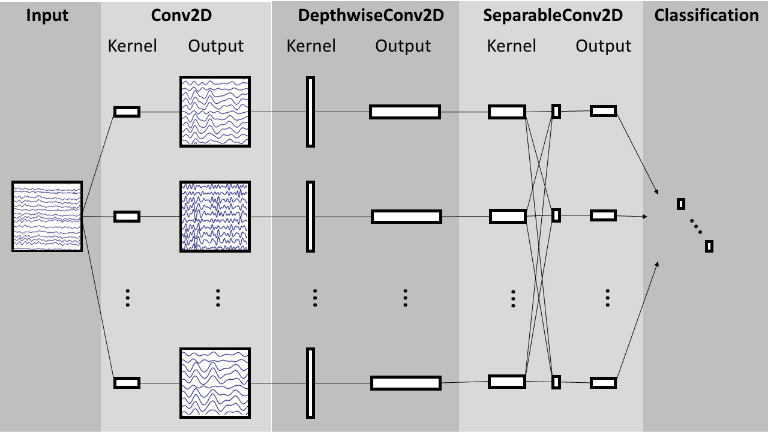
\includegraphics[width=0.90\textwidth]{img/eegnet_arch.png}
    %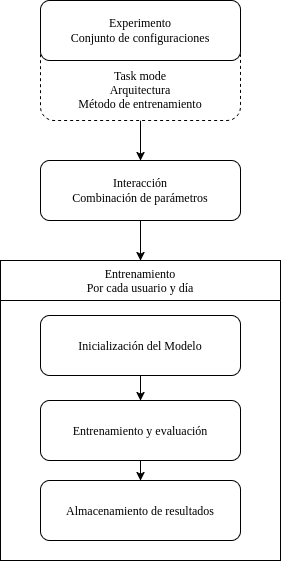
\includegraphics[height=\dimexpr\pagegoal-\pagetotal-\baselineskip\relax,width=\textwidth,keepaspectratio]{img/diagrama_pipeline.drawio.png}
    \caption{Arquitectura de EEGNet. las lineas muestran la conexión entre las capas \cite{lawhern_EEGNetCompact2018}.}
    \label{fig:eegnet_arch}
\end{figure}


Estudios posteriores han mostrado que EEGNet es capaz de aprender representaciones similares a las obtenidas mediante métodos clásicos de extracción de características, como Filter Bank Common Spatial Patterns (FBCSP), manteniendo la ventaja de realizar dicho proceso de forma automática dentro de la propia red neuronal. Finalmente, esta arquitectura ha mostrado buenos resultados al clasificar potenciales en la señal EEG relacionados con el movimiento (\acrshort{mrcp}) \cite{lawhern_EEGNetCompact2018,kollod_DeepComparisons2023}.

La elección de este modelo se debe principalmente a su arquitectura compacta y a su capacidad para obtener buenos resultados incluso con conjuntos de datos reducidos, una situación habitual en aplicaciones basadas en \acrshort{eeg}. Además, el uso de convoluciones \textit{Depthwise} y \textit{Separable} permite reducir significativamente el número de parámetros del modelo respecto a otras arquitecturas convolucionales, disminuyendo así el el coste computacional del entrenamiento \cite{lawhern_EEGNetCompact2018}.

{\color{red}

Para cada uno:

breve descripción (2-3 líneas)

por qué lo eliges

NO pongas la arquitectura entera en detalle aquí (eso es más de anexos si acaso)
}